\subsection{Prophet Executor}\label{subsec: processor-prophet-executor}
prophet用$\texttt{\%\{ ... \%\}}$ 来表示。prophet被执行不影响pc、fp寄存器存储的地址。但是会更改vm保存在内存中的变量值。
下边是一个prophet的例子:
\begin{lstlisting}[label={lst:prophet-demo}]
fn main() {
    let a = 3
    // Use custom prophet to print the value of a
    // local 用来获取函数中的变量,用来进行和vm通信
    %{print(local.a)%}
}
\end{lstlisting}

虚拟机如何处理prophets

为了能够正确处理prophets,虚拟机会实现两个方法: `binding\_prophet` 和 `execute\_prophet` 。

`binding\_prophet` 主要作用是将用户合约中写的prophets和虚拟机中采用rust实现的对应方法进行绑定,并且获取对应的prophet参数进行处理。

`execute\_prophet` 用于执行用户合约中编写的写的prophets,prophets的执行会优先于虚拟机指令的执行。

虚拟机执行编译后的程序的过程如下:
下图是虚拟机执行编译后的程序的示意图\ref{fig: prophet-flow}:
\begin{figure}[!htp]
    \centering
    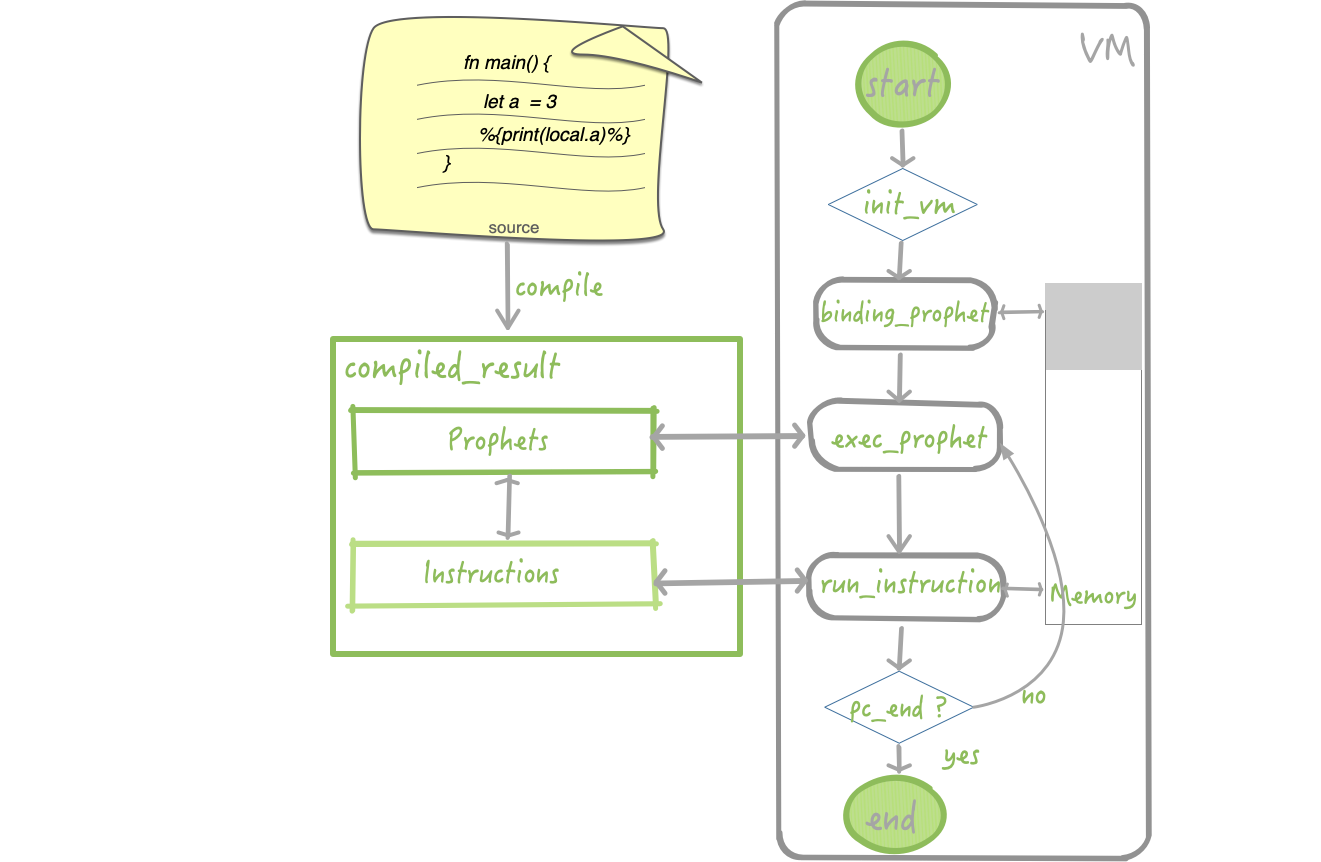
\includegraphics[width=0.8\textwidth]{prophet-flow}
    \caption{OlaVM prophets执行流程图}
    \label{fig: prophet-flow}
\end{figure}

\emph{binding\_prophet}

该方法在执行前调用,该方法有以下参数:

\begin{itemize}
    \item String 形式的  prophet code
    \item prophet 中定义的变量名称与对应合约编译后json中的引用id号的HashMap
    \item 应用id号对应的ProphetReference的HashMap
\end{itemize}

该方法返回一个dynamic structure,后续会被 `execute\_prophet` 方法使用

\emph{execute\_prophet}

当有提示要执行时,这个方法会在每个虚拟机步骤的开始被调用。它接收由binding\_prophet创建的动态结构以及程序常量和一组包含对虚拟机内部的有限访问的代理。

\begin{itemize}
    \item binding\_prophet 返回的动态结构, 包含变量以及code以及内存索引内容
    \item vm 的不可变引用,vm这个结构包含了内存段管理器和运行上下文的可变引用等内容
\end{itemize}

\emph{变量值如何在prophets和vm中传递}

每个程序中的变量的地址和值都可以通过ProphetReference 结构获取数据,prophet processor提供了访问变量值(value)和地址(ptr)的辅助函数